\documentclass[pdftex]{beamer}
%\documentclass[notes=show]{beamer}
%\documentclass[xcolor=dvipsnames]{beamer}

\usepackage{amssymb}
\usepackage{latexsym}
\usepackage{amsfonts}
\usepackage{amsmath}
\usepackage[absolute,overlay]{textpos}
\usepackage[english]{babel}
\usepackage[latin1]{inputenc}
%\usepackage{times}
\usepackage[T1]{fontenc}
\usepackage{tabularx}
\newcolumntype{Y}{>{\small\raggedright\arraybackslash}X}
\usepackage{graphicx}
\usepackage{bigstrut}
\usepackage{bbm}
\usepackage{mathrsfs}
\usepackage{epsfig}
\usepackage{array}
%\usepackage{natbib}
\usepackage{ulem}
\mode<presentation> {
%\usetheme[left,width=1.7cm]{Berkeley}
%\usetheme{default}
\usetheme{Boadilla}
  \usecolortheme[RGB={103,102,204}]{structure}
%\usecolortheme{dove}
  \useoutertheme{infolines}
  \setbeamercovered{transparent}
 }

%\renewcommand{\familydefault}{cmss}
%\renewcommand{\mathrm}{\mathsf}
%\renewcommand{\textrm}{\textsf}
\usefonttheme{serif}
\newcommand{\X}{{\mathbf{X}}}
\newcommand{\x}{{\mathbf{x}}}
\newcommand{\E}{\mathsf{E}}
\newcommand{\V}{\mathsf{Var}}


    %%%%%%%%%%%%%%%%%%%%%%%%%%%%%%%%%%%%%%%%%%%%%%%%%%%%%%%%%%%%%%%%%%%%%%%%%%%%%%
    %         Neue Kommandos f�r fette Mathebuchstaben innerhalb von Formeln     %
    %%%%%%%%%%%%%%%%%%%%%%%%%%%%%%%%%%%%%%%%%%%%%%%%%%%%%%%%%%%%%%%%%%%%%%%%%%%%%%
    \newcommand{\bom}{\boldmath}
    \newcommand{\ubom}{\unboldmath}
    \newcommand{\mb}{\mathbf}

    \newcommand{\fmalpha}{\mbox{\bom${\alpha}$}}               %Fettes alpha
    \newcommand{\fmbeta}{\mbox{\bom${\beta}$}}                 %Fettes beta
    \newcommand{\fmgamma}{\mbox{\bom${\gamma}$}}               %Fettes gamma
    \newcommand{\fmdelta}{\mbox{\bom${\delta}$}}               %Fettes delta
    \newcommand{\fmepsilon}{\mbox{\bom${\epsilon}$}}           %Fettes epsilon
    \newcommand{\fmvarepsilon}{\mbox{\bom${\varepsilon}$}}     %Fettes varepsilon
    \newcommand{\fmzeta}{\mbox{\bom${\zeta}$}}                 %Fettes zeta
    \newcommand{\fmeta}{\mbox{\bom${\eta}$}}                   %Fettes eta
    \newcommand{\fmta}{\mbox{\bom${\theta}$}}                  %Fettes theta (ta)
    \newcommand{\fmvarta}{\mbox{\bom${\vartheta}$}}         	 %Fettes vartheta (ta)
    \newcommand{\fmiota}{\mbox{\bom${\iota}$}}                 %Fettes iota
    \newcommand{\fmkappa}{\mbox{\bom${\kappa}$}}               %Fettes kappa
    \newcommand{\fmla}{\mbox{\bom${\la}$}}                     %Fettes lambda (la)
    \newcommand{\fmmu}{\mbox{\bom${\mu}$}}                     %Fettes mu
    \newcommand{\fmnu}{\mbox{\bom${\nu}$}}                     %Fettes nu
    \newcommand{\fmxi}{\mbox{\bom${\xi}$}}                     %Fettes xi
    \newcommand{\fmo}{\mbox{\bom${\o}$}}                       %Fettes o
    \newcommand{\fmpi}{\mbox{\bom${\pi}$}}                     %Fettes pi
    \newcommand{\fmvarpi}{\mbox{\bom${\varpi}$}}               %Fettes varpi
    \newcommand{\fmrho}{\mbox{\bom${\rho}$}}                   %Fettes rho
    \newcommand{\fmvarrho}{\mbox{\bom${\varrho}$}}             %Fettes varrho
    \newcommand{\fmsigma}{\mbox{\bom${\sigma}$}}               %Fettes sigma
    \newcommand{\fmvarsigma}{\mbox{\bom${\varsigma}$}}         %Fettes varsigma
    \newcommand{\fmtau}{\mbox{\bom${\tau}$}}                   %Fettes tau
    \newcommand{\fmupsilon}{\mbox{\bom${\upsilon}$}}           %Fettes upsilon
    \newcommand{\fmphi}{\mbox{\bom${\phi}$}}                   %Fettes phi
    \newcommand{\fmvarphi}{\mbox{\bom${\varphi}$}}             %Fettes varphi
    \newcommand{\fmchi}{\mbox{\bom${\chi}$}}                   %Fettes chi
    \newcommand{\fmpsi}{\mbox{\bom${\psi}$}}                   %Fettes psi
    \newcommand{\fmomega}{\mbox{\bom${\omega}$}}               %Fettes omega
    \newcommand{\fmimath}{\mbox{\bom${\imath}$}}               %Fettes imath


\setbeamercolor{bibliography entry title}{fg=black}
\setbeamercolor{bibliography entry author}{fg=black}
\setbeamercolor{subsection in toc}{fg=structure}
\setbeamercolor{palette primary}{bg=structure, fg=white}
%\setbeamercolor{palette secondary}{bg=structure, fg=black}
%\setbeamercolor{palette tertiary}{bg=structure, fg=black}
\setbeamercolor{caption name}{fg=black} \setbeamersize{text margin
left=.8cm} \setbeamersize{text margin right=1cm}
\hypersetup{linkbordercolor={1 0 0}} \setbeamertemplate{navigation
symbols}{} \setbeamertemplate{headline}[default]

\setbeamertemplate{enumerate items}[default]

\newcounter{transfct}
\newcounter{begbs}
\newcounter{endbs}
\title[Introduction]{Econometrics 2 (Part 2)}

\author[Lychagin  \& Mu\c co]{Arieda Mu\c co}
\institute[CEU]{Central European University}
\date{Spring 2020}


\AtBeginSection[] {
  \begin{frame}<handout:0>
    \frametitle{TOC}
    \tableofcontents[currentsection]
  \end{frame}
}

%\AtBeginSubsection[] {
%  \begin{frame}<beamer>
%   \frametitle{Outline}
%    \tableofcontents[currentsection,currentsubsection]
%  \end{frame}
%}

%\beamerdefaultoverlayspecification{<+->}

\pgfdeclareimage[height=.7cm]{logo}{rgs2}
\logo{\pgfuseimage{logo}}
\begin{document}

\frame{\titlepage}


\begin{frame}
\frametitle{Contact}
\begin{itemize}
\item Sergey Lychagin: \href{mailto:LychaginS@ceu.edu}{LychaginS@ceu.edu}\\
\sout{Office: Budapest campus, Nador 13, 513}
\item Arieda Mu\c co: \href{mailto:MucoA@ceu.edu}{MucoA@ceu.edu}\\
\sout{Office:  Budapest campus, Nador 13, 507}
\item Boldizs\'ar Juh\'asz (TA): \href{mailto:juhasz_boldizsar@phd.ceu.edu}{juhasz\_boldizsar@phd.ceu.edu}
\end{itemize}

\end{frame}

\begin{frame}
\frametitle{Textbooks}
\begin{itemize}
\item Introductory Econometrics: A Modern Approach by Wooldridge
\item Mostly Harmless Econometrics by Angrist and Pischke
\item \textcolor{blue}{Mastering Metrics by Angrist and Pischke}
\item \textcolor{blue}{Casual Inference: The Mixtape by Cunningham}
\item Reading list of applied papers
\end{itemize}
\end{frame}


\begin{frame}
\frametitle{Outline: Tentative Schedule}
\begin{enumerate}
\item Economic research questions: causality
\item The experimental ideal
\item Linear regression
\item Instrumental Variables
\item Panel Data, Fixed Effects, Differences-in-Differences
\item Matching
\item Program Evaluation: Nonparametric Methods
\item \textcolor{blue}{Regression Discontinuity}
\end{enumerate}
\end{frame}


 \frame{ \frametitle{Della Vigna and Card}
\begin{center}
\begin{figure}

\includegraphics[width=1\linewidth]{graphs/what_economist_do.png}
\end{figure}
\end{center}
 }
 
 \frame{ \frametitle{}
\begin{center}
\begin{figure}
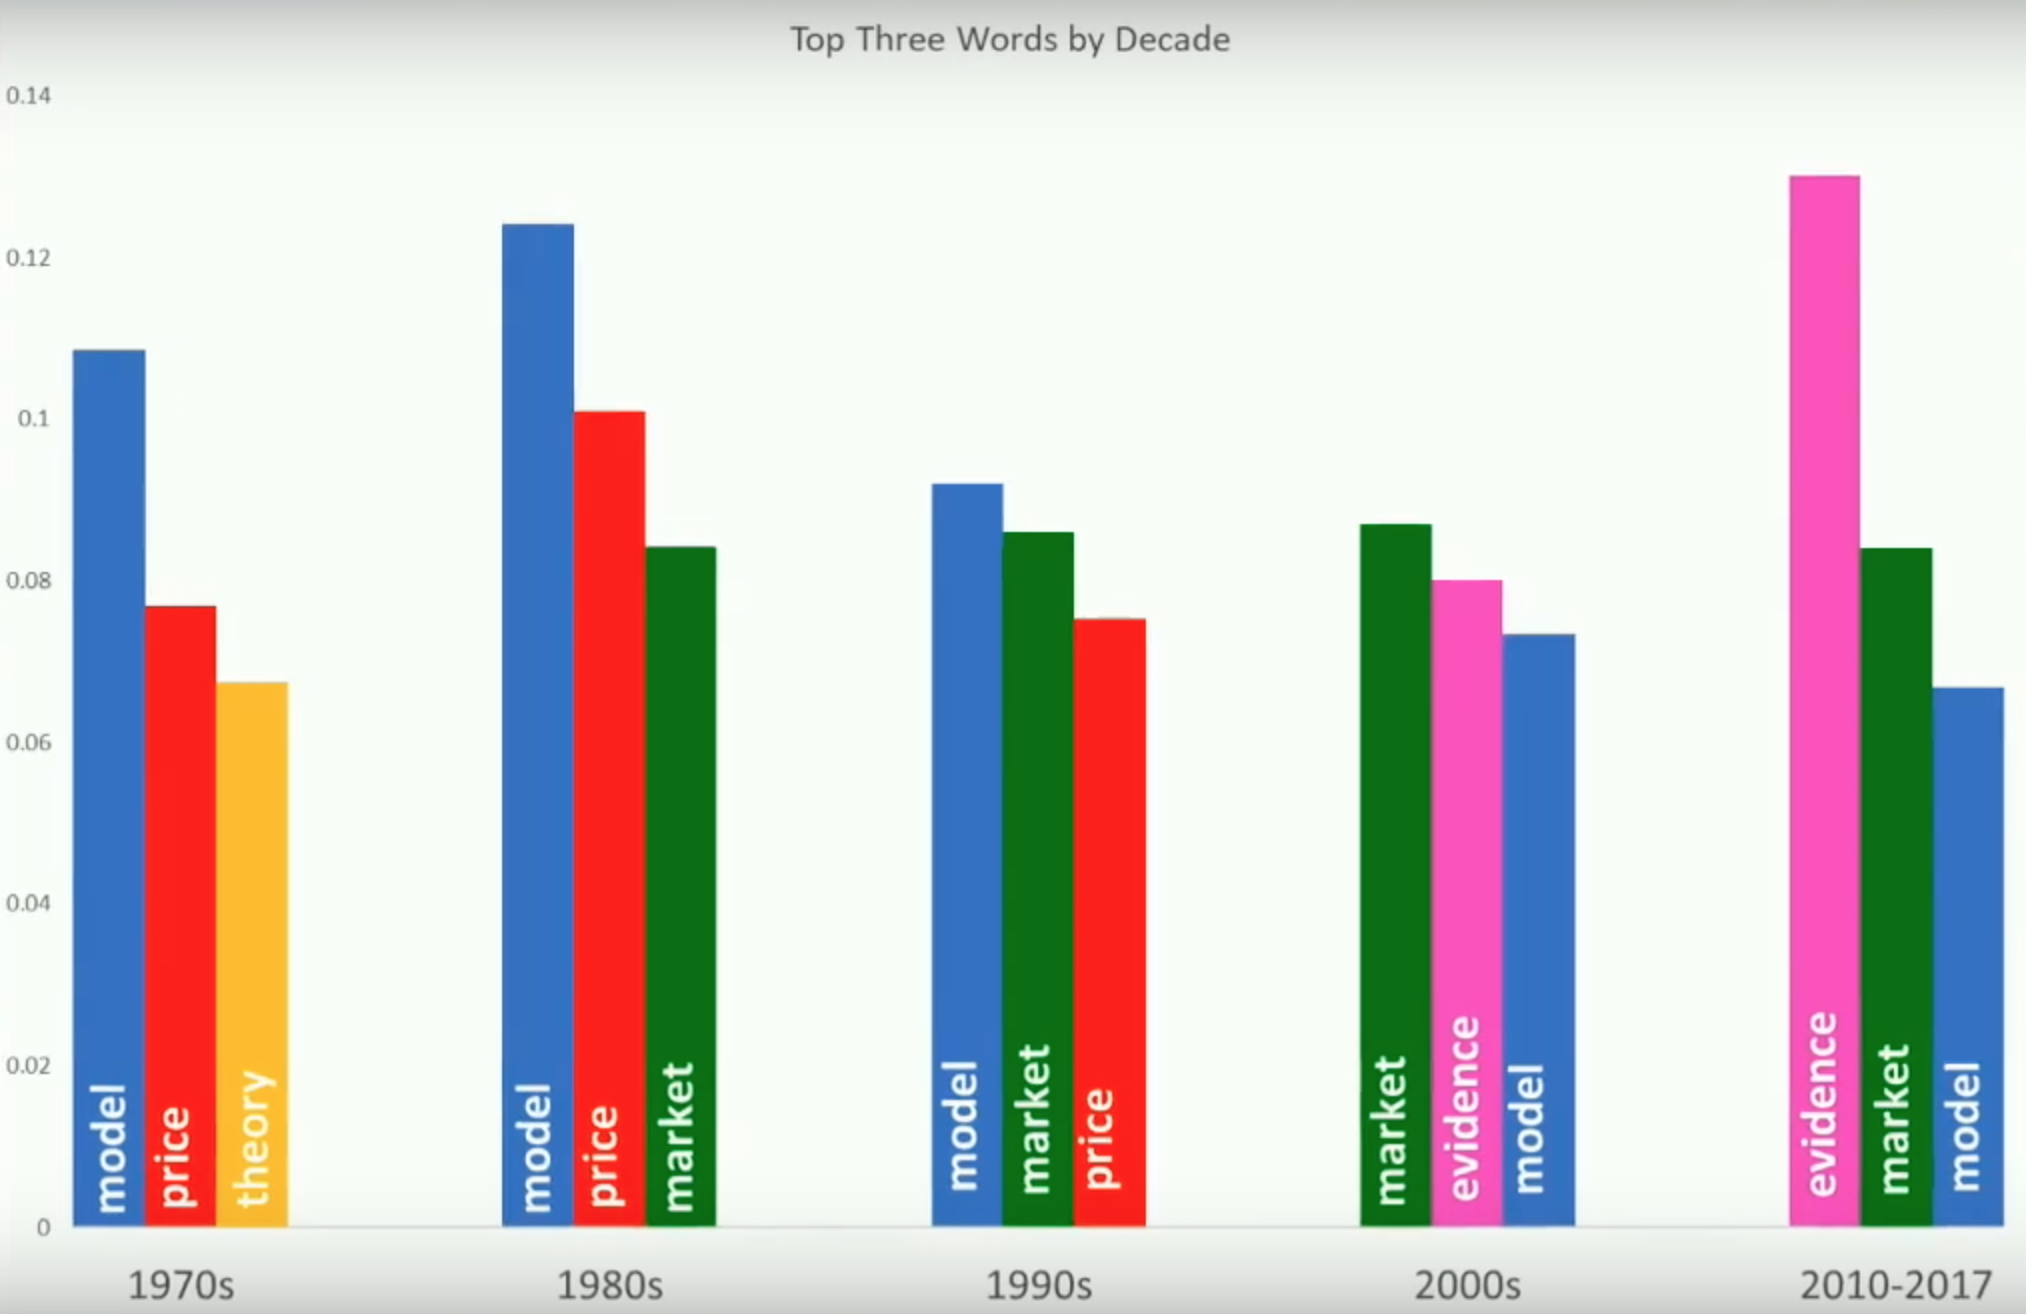
\includegraphics[width=1\linewidth]{graphs/what_economist_do1.png}
\end{figure}
\end{center}
 }

 \frame{ \frametitle{Applied Microeconometrics Papers}
\begin{center}
\begin{figure}

\includegraphics[width=1\linewidth]{graphs/what_economist_do2.png}
\end{figure}
\end{center}
 }

\frame{ \frametitle{}
\begin{center}
\begin{figure}

\includegraphics[width=0.8\linewidth]{graphs/detective.png}
\end{figure}
\end{center}
}
 
\begin{frame}
\frametitle{Statistical Models of Shoe and Leather}
Freedman, David A. (1991) "Statistical Models and Shoe Leather", Sociological Methodology, 21, 291-313
\bigskip

John Snow studies of the cholera epidemics in Europe in the 19th century and proves that cholera is a waterborne infectious disease

\begin{itemize}
  \item In the $19^{th}$ century no microbiology, limited microscopes
  \item Theory: diseases result from "poison in the air" - miasma
  \item Cholera Europe in epidemic waves
  \item Snow studied spatial pattern of epidemics along tracks of human commerce
  \item Influence of water supply on incidence of Cholera?
\end{itemize}
\end{frame}


\begin{frame}
\frametitle{Is cholera a waterborne or an airborne disease?}

London in the 1800's: different water companies serve different areas

\begin{itemize}
  \item Some companies take water from the Thames polluted by sewage
  \item 2 companies
  \begin{itemize}
  \item Southwark \& Vauxhall: downstream from sewage discharges
  \item Lambeth: intake point upstream
  \end{itemize}

  \item Both companies served the same parts of London during the 1853-54 cholera epidemic
  \item Sometimes houses next to each other in the same street were served by the 2 different companies
    \begin{itemize}

  \item Each company supplies rich and poor, large and small houses, no difference in condition or occupation
  \end{itemize}
  \item Idea: compare number of cholera victims
\end{itemize}
\end{frame}

\begin{frame}
\frametitle{Method of Shoe and Leather}

\begin{itemize}
  \item Snow surveyed houses in large parts of London
  \item Water company
  \item Cholera victims
  \item 300,000 households involved
  \item Reward: clear result
\end{itemize}
\end{frame}

 \frame{ \frametitle{}
\begin{center}
\begin{figure}
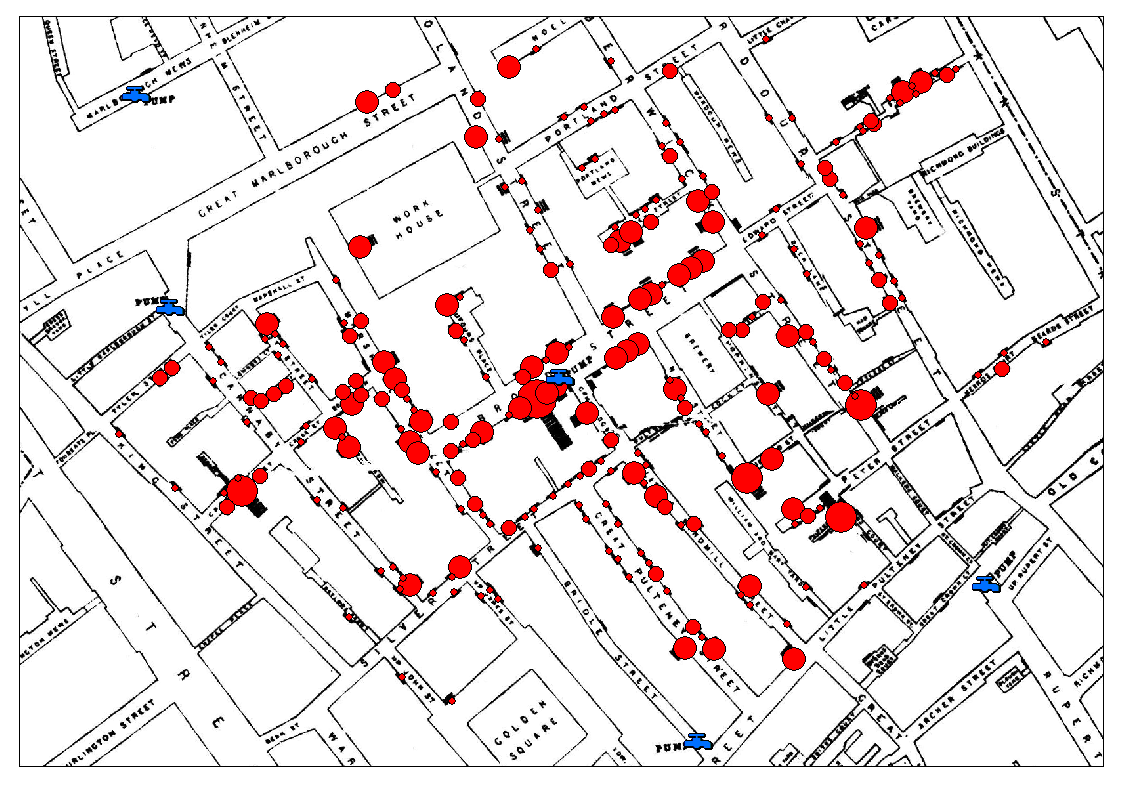
\includegraphics[width=1\linewidth]{graphs/SnowMap_Points.png}
\end{figure}
\end{center}
 }
 

 

 
\frame{ \frametitle{}
\begin{center}
\begin{figure}[t]
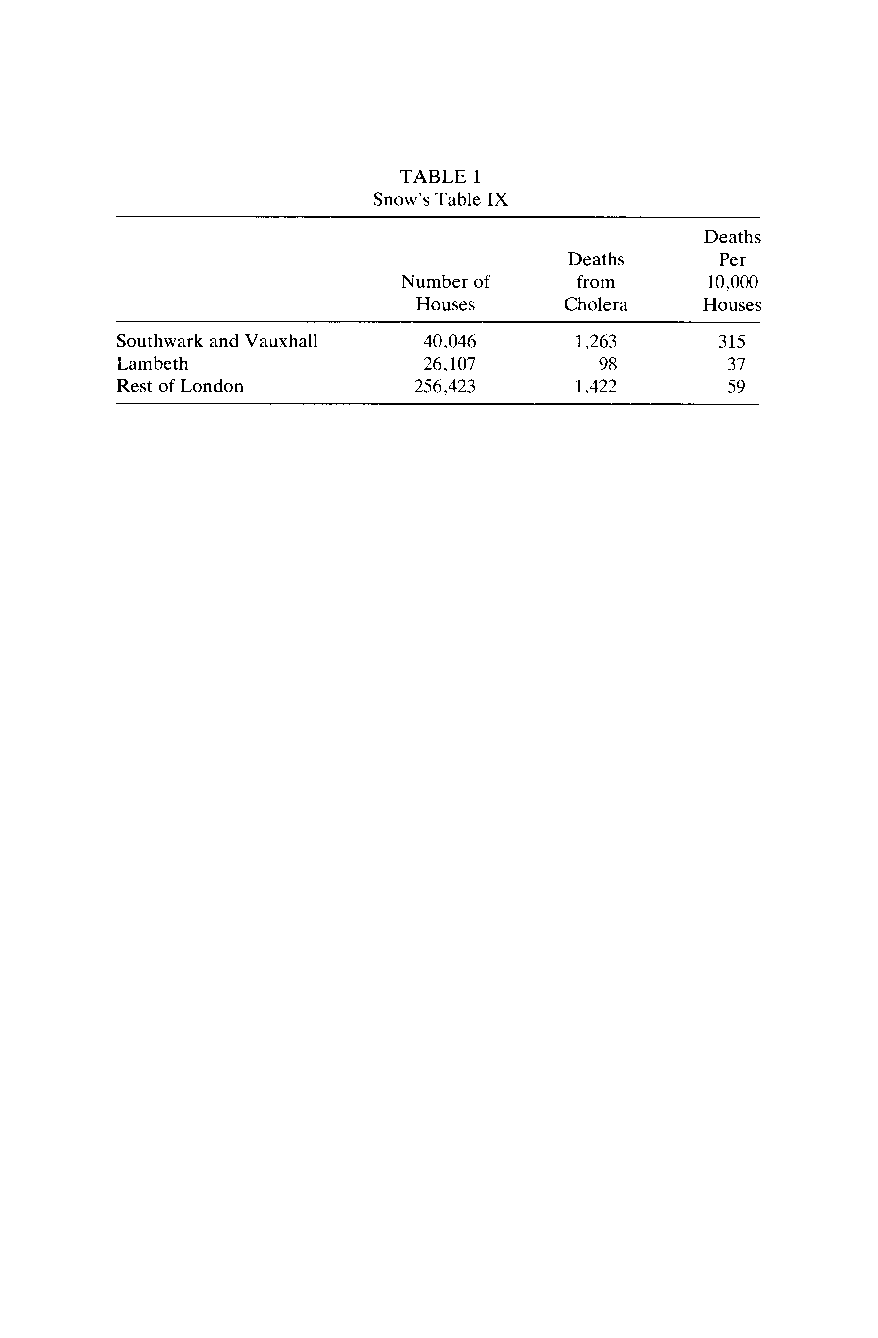
\includegraphics[width=1.1\linewidth]{graphs/freedman_tab1.pdf}
\end{figure}
\end{center}
 }

\begin{frame}
\frametitle{The Experimental Ideal}

Social experiment is the most influential research design. Why?
\bigskip

Solves Selection Problem
\end{frame}




   \begin{frame}
\frametitle{Potential Outcome Model}
$D_i=\{0,1 \}$ treatment variable (hospital care)

For each population unit $i$ we consider two \emph{potential outcomes} (health status)
\[\begin{array}{cl}
    Y_{1i} & \text{outcome with treatment} \\
    Y_{0i} & \text{outcome without treatment}
  \end{array}
\]
The gain from treatment or \emph{causal effect} for unit $i$ is
\[ Y_{i1}-Y_{i0} \]
Problem: For each $i$, only one of  $ Y_{i1}$ or $Y_{i0}$ is observed.

%\emph{Missing data problem}

\end{frame}

\begin{frame}
\frametitle{Observed outcome}

We observe
\begin{eqnarray*}
Y_i  &=& \left\{ \begin{array}{cc}
                                                Y_{1i} & \text{if}\;\; D_i=1 \\
                                                Y_{0i} & \text{if}\;\; D_i=0
                            \end{array}
                            \right. = Y_{0i}+ (Y_{1i}-Y_{0i}) D_i
\end{eqnarray*}


In the population distribution of $Y_{1i}$ and $Y_{0i}$, we can compare the average health of \emph{treated} and \emph{non-treated}


\begin{eqnarray*}
  \underset{\text{observed difference}}{\underbrace{E[Y_i|D_i=1]-E[Y_i|D_i=0]}} &=&  \\
  \underset{\text{average treatment effect}}{\underbrace{E[Y_{1i}|D_i=1]-E[Y_{0i}|D_i=1]}}  &+& \underset{\text{selection bias}}{\underbrace{E[Y_{0i}|D_i=1]-E[Y_{0i}|D_i=0] }}
\end{eqnarray*}

\end{frame}


\begin{frame}\tiny

\frametitle{Observed outcome}

Remind that the observed difference is $E[Y_{i}|D_i=1]-E[Y_{i}|D_i=0]$\\
Which can be rewritten as:
\[
E[\underbrace{Y_{0i}+ (Y_{1i}-Y_{0i}) D_i}_{\text{$Y_i$ }}|D_i=1]-E[\underbrace{Y_{0i}+ (Y_{1i}-Y_{0i}) D_i}_{\text{$Y_i$ }}|D_i=0]
\]
From the properties of the conditional expectation we can rearrange the above equation as:
\begin{equation*}
E[Y_{0i}|D_i=1]+E [(Y_{1i}-Y_{0i}) D_i|D_i=1]-E[Y_{0i}|D_i=0]-E[(Y_{1i}-Y_{0i}) D_i|D_i=0]
\end{equation*}

Which can be rewritten as:
\[
E[Y_{0i}|D_i=1]+E [(Y_{1i}-Y_{0i})|D_i=1]-E[Y_{0i}|D_i=0]
\]
And is equivalent to:

\[
E[Y_{0i}|D_i=1]+E [Y_{1i}| D_i=1]-E[Y_{0i}|D_i=1]-E[Y_{0i}|D_i=0]
\]
Rearranging we get:

\begin{eqnarray*}
  \underset{\text{average treatment effect}}{\underbrace{E[Y_{1i}|D_i=1]-E[Y_{0i}|D_i=1]}}  &+& \underset{\text{selection bias}}{\underbrace{E[Y_{0i}|D_i=1]-E[Y_{0i}|D_i=0] }}
\end{eqnarray*}
\end{frame}




\begin{frame}
\frametitle{Random assignment as a solution}

Random assignment makes $D_i$ independent of the potential outcome. If $D_i$ is independent of $Y_i$ then $E[Y_i|D_i]=E[Y_i|D_i=1]=E[Y_i|D_i=0]=E[Y_i]$ 
\begin{eqnarray*}
E[Y_i|D_i=1]-E[Y_i|D_i=0]  &=& E[Y_{1i}|D_i=1]-E[Y_{0i}|D_i=0] \\
        &=& E[Y_{1i}|D_i=1]-E[Y_{0i}|D_i=1]  \\
         &=& E[Y_{1i}-Y_{0i}|D_i=1]=E[Y_{1i}-Y_{0i}] \\
\end{eqnarray*}
The observed difference in mean outcomes equals the \emph{average treatment effect}.
Examples:
\begin{itemize}
  \item health treatments
  \item government sponsored training programs
  \item education production: effect of class size, teacher quality, etc. on  student achievement
\end{itemize}

\end{frame}

 
 \begin{frame}
\frametitle{Regression Analysis of Experiments}
Assume $Y_{i1}-Y_{i0} = \rho$ \emph{constant} treatment effect
\begin{eqnarray*}
 Y_i &=&  \alpha + \rho D_i + \eta_i
\end{eqnarray*}

\begin{eqnarray*}
 E[Y_i|D_i=1] &=&  \alpha + \rho  +  E[\eta_i|D_i=1] \\
 E[Y_i|D_i=0] &=&  \alpha  +  E[\eta_i|D_i=0]\\
 E[Y_i|D_i=1]-E[Y_i|D_i=0]&=&    \rho +  \underset{\text{selection bias}}{\underbrace{E[\eta_i|D_i=1]-E[\eta_i|D_i=0]}}
\end{eqnarray*}
Selection bias amounts to correlation between regression error $\eta_i$ and $D_i$.
\end{frame}


 \begin{frame}
\frametitle{Regression Analysis of Experiments}
We know about the selection bias
\begin{eqnarray*}
 E[\eta_i|D_i=1]-E[\eta_i|D_i=0]= E[Y_{0i}|D_i=1]-E[Y_{0i}|D_i=0]
\end{eqnarray*}
If $D_i$ is randomly assigned, the selection bias is equal to zero.

Thus estimating the regression model results in the \emph{causal effect} $\rho$.
\bigskip

Regression model with covariates
\begin{eqnarray*}
 Y_i &=&  \alpha + \rho D_i + \beta X_i+ \eta_i
\end{eqnarray*}
If $X_i$ uncorrelated with $D_i$, including them will not affect estimate of $\rho$, but increase precision.

\end{frame}

\end{document}


